%
% gammareflektion.tex
%
% (c) 2021 Prof Dr Andreas Müller, OST Ostschweizer Fachhochschule
%
\subsection{Reflektionsformel für die Gamma-Funktion
\label{buch:funktionentheorie:subsection:gammareflektion}}
Die Formel~\eqref{buch:rekursion:gamma:spiegelung-betaintegral}
stellt eine Beziehung zwischen dem Produkt $\Gamma(x)\Gamma(1-x)$
von zwei Werten der Gamma-Funktion in Punkten der komplexen Ebene,
die durch Spiegelung an der Geraden $\operatorname{Re}x=\frac12$
auseinander hervorgehen, und einem speziellen Beta-Integral her.

\begin{satz}
\index{Satz!Spiegelungsformel für $\Gamma(x)$}%
\label{buch:funktionentheorie:satz:spiegelungsformel}
Für $0<x<1$ gilt
\begin{equation}
\Gamma(x)\Gamma(1-x)
=
\frac{\pi}{\sin\pi x}.
\end{equation}
\index{Gamma-Funktion!Spiegelungsformel}%
\end{satz}

\begin{figure}
\centering
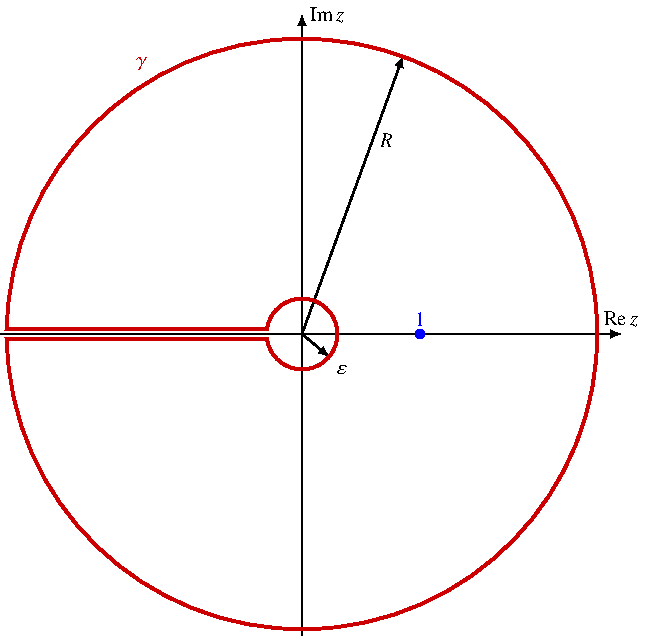
\includegraphics{chapters/080-funktionentheorie/images/gammapfad.pdf}
\caption{Pfad zur Auswertung des
Integrals~\eqref{buch:funktionentheorie:eqn:gammapfadintegral}
mit Hilfe des Residuensatzes.
\label{buch:funktionentheorie:fig:gammapfad}}
\end{figure}

\begin{proof}[Beweis]
In der Formel~\eqref{buch:rekursion:gamma:spiegelung-betaintegral}
wurde bereits ein Zusammenhang zwischen $\Gamma(x)\Gamma(1-x)$
und einem Beta-Integral hergestellt, konkret
\[
\Gamma(x)\Gamma(1-x)
=
B(x,1-x)
=
\int_0^1 t^{x-1}(1-t)^{-x}\,dt.
\]
Mit der Substitution $t=s/(s+1)$, die bereits für die Herleitung der
Formel~\eqref{buch:rekursion:gamma:beta:sinf} verwendet wurde, ergibt sich
\[
\Gamma(x)\Gamma(1-x)
=
\int_0^\infty 
\frac{s^{x-1}}{s+1}
\,ds.
\]
Um dieses Integral zu berechnen, verwenden wir den Cauchy-Integralsatz,
um das Integral
\begin{equation}
I
=
\oint_\gamma \frac{z^{x-1}}{1-z}\,dz
\label{buch:funktionentheorie:eqn:gammapfadintegral}
\end{equation}
zu berechnen.
Darin hat die Funktion im Zähler des Integranden $f(z)=z^{x-1}$ 
nur ausserhalb der negativen reellen Achse einen wohldefinierten Wert.
In Polarkoordinaten $z=re^{i\varphi}$ verwenden wir
den Hauptwert $z^{x-1}=r^{x-1}e^{i(x-1)\varphi}$.
Aus dem Cauchy-Integralsatz lesen wir den Wert
\[
I = 2\pi i
\]
ab.

Das Integral \eqref{buch:funktionentheorie:eqn:gammapfadintegral}
kann zerlegt werden in die Integrale
\begin{align*}
I
&=
I_R+I_++I_\varepsilon+I_-,
\end{align*}
wobei $I_R$ das Integral über den äusseren Kreis vom Radius $R$ ist,
$I_\varepsilon$ das Integral im Gegenuhrzeigersinn über den inneren Kreis
vom Radius $\varepsilon$.
Die Terme $I_{\pm}$ sind die Integrale entlang der negativen
reellen Achse, wobei das Pluszeichen für den oberen $-R$ nach
$-\varepsilon$ gelten soll.

Für die beiden Integrale $I_R$ und $I_\varepsilon$ wird die Parametrisierung
$\varphi\mapsto z(\varphi) = re^{i\varphi}$ mit $dz=ire^{i\varphi}\,d\varphi$
verwendet.
Das Integral über den Kreis vom Radius $r$ im Gegenuhrzeigersinn ist
\begin{align*}
I_r
&=
\int_{-\pi}^\pi
\frac{r^{x-1}e^{i(x-1)\varphi}}{1-re^{i\varphi}} ire^{i\varphi}\,d\varphi
=
i\int_{-\pi}^\pi
\frac{r^xe^{ix\varphi}}{1-re^{i\varphi}}
\,d\varphi
\end{align*}
Die beiden Teile $I_R$ und $I_\varepsilon$ können wie folgt noch
weiter vereinfacht werden:
\begin{align*}
\\
I_R
&=
iR^{x-1}
\int_{-\pi}^\pi
\frac{e^{ix\varphi}}{1/R-e^{i\varphi}}
\,d\varphi
\\
I_{\varepsilon}
&=
-
i
\varepsilon^x
\int_{\pi}^{-\pi}
\frac{e^{ix\varphi}}{1-\varepsilon e^{i\varphi}}
\,d\varphi,
\end{align*}
wobei das negative Zeichen bei $I_\varepsilon$ daher rührt, dass der
kleine Kreis im Uhrzeigersinn durchlaufen wird.
Für grosse Werte von $R$ ist das erste Integral beschränkt, aber wegen
$x-1<0$ konvergiert der Vorfaktor $R^{x-1}$ gegen 0 für $R\to\infty$.
Ähnlich ist das zweite Integral für kleine $\varepsilon$ beschränkt, aber
$\varepsilon^x$ konvergiert gegen $0$ für  $\varepsilon\to 0$.
Wir können daher
\begin{align*}
\lim_{R\to\infty}
I_R
&=
\lim_{R\to\infty}
R^{x-1}
\int_{-\pi}^\pi
\frac{e^{i(x-1)\varphi}}{1/R-e^{i\varphi}}
ie^{i\varphi}
\,d\varphi
=0
\\
\text{und}
\qquad
\lim_{\varepsilon\to 0}
I_\varepsilon
&=
-
\lim_{\varepsilon\to 0}
\int_{\pi}^{-\pi}
\frac{\varepsilon^{x-1}e^{i(x-1)\varphi}}{1-\varepsilon e^{i\varphi}}
i\varepsilon e^{i\varphi}
\,d\varphi
=
0
\end{align*}
folgern.

Die anderen zwei Integrale verwenden die Parametrisierung
$z(s) = -s = se^{\pm i\pi}$ mit $dz = e^{\pm i\pi}\,ds$.
Damit werden sie
\begin{align*}
I_+
&=
\int_{R}^{\varepsilon}
\frac{s^{x-1}e^{i(x-1)\pi}}{1-se^{i\pi}}
e^{i\pi}
\,ds
=
\int_{\varepsilon}^R
\frac{s^{x-1}e^{ix\pi}}{1+s}
\,ds
\\
I_-
&=
\int_{\varepsilon}^{R}
\frac{s^{x-1}e^{i(x-1)(-\pi)}}{1-se^{-i\pi}}
e^{-i\pi}
\,ds
=
-
\int_{\varepsilon}^{R}
\frac{s^{x-1}e^{-ix\pi}}{1+s}
\,ds.
\intertext{Die beiden Integrale stimmen bis auf den von $t$ unabhängigen
Faktor $e^{\pm ix\pi}$ überein, sie können daher zusammegefasst werden zu}
I_++I_-
&=
(e^{ix\pi}-e^{-ix\pi})
\int_{\varepsilon}^{R}
\frac{s^{x-1}}{1+s}
\,ds
=
\frac{e^{ix\pi}-e^{-ix\pi}}{2i}
\cdot
2i \int_{\varepsilon}^{R}
\frac{s^{x-1}}{1+s}
\,ds
\\
&=
2i
\sin(\pi x)
\int_{\varepsilon}^R
\frac{s^{x-1}}{1+s}
\,ds.
\end{align*}
Durch Grenzübergang $R\to\infty$ und $\varepsilon \to 0$ wird dies zu
\[
I
=
2i\sin(\pi x) \int_{0}^\infty \frac{s^{x-1}}{1+s}\,ds
\]
Zusammen mit dem früher bestimmten Wert $I=2\pi i$ folgt 
\[
2\pi i
= 
2i\sin(\pi x)
\int_{0}^\infty \frac{s^{x-1}}{1+s}\,ds
\qquad\Rightarrow\qquad
\frac{\pi}{\sin \pi x}
=
\int_{0}^\infty \frac{s^{x-1}}{1+s}\,ds
=
\Gamma(x)\Gamma(1-x).
\]
Damit ist der Satz bewiesen.
\end{proof}

